\chapter{Introducci\'on a la expresi\'on referencial}
\label{sec:intro}
%tesis en linguistica http://elies.rediris.es/miscelanea/misce_9/alcina.pdf

%En este cap\'itulo daremos una introducci\'on al problema de la generaci\'on autom\'atica de expresiones referenciales, contaremos las contribuciones de este trabajo y mostraremos como est\'a organizada la tesis.


La generaci\'on de lenguaje natural (GLN) es el proceso de construcci\'on de un texto en lenguaje natural, para la comunicaci\'on con fines espec\'ificos. El proceso de convertir autom\'aticamente la informaci\'on no ling\"u\'{i}stica (por ejemplo, a partir de una base de datos como se muestra en la Tabla \ref{tabla-propiedades}) a texto en lenguaje natural, es \'util para aplicaciones pr\'acticas que van desde la generaci\'on de pron\'osticos del tiempo, a resumir informaci\'on m\'edica~\cite{dale2000}. La generaci\'on autom\'atica de expresiones referenciales es una sub\'area de la generaci\'on de lenguaje natural, la cual es una rama principal de la inteligencia artificial. Cuando hablamos, nos referimos a cosas, es decir usamos expresiones referenciales, un sistema que genera texto, tambi\'en deber\'a generar expresiones referenciales.


Un sistema de generaci\'on autom\'atica de texto en lenguaje natural deber\'ia incluir m\'inimamante 
las tareas de \emph{determinaci\'on de contenido} (qu\'e decir), \emph{lexicalizaci\'on} (con qu\'e palabras), y la \emph{realizaci\'on ling\"{u}\'istica} (armar el  sintagma nominal para que sea gramaticalmente correcto). \\
En generaci\'on autom\'atica de expresiones referenciales, tenemos esas 3 partes tambi\'en: la determinaci\'on de contenido est\'a dada por las propiedades o relaciones del objeto que queremos incluir en la expresi\'on referencial, la lexicalicalizaci\'on de las anteriores, es decir las palabras que vamos a usar para nombrarlo y la realizaci\'on ling\"u\'istica, que se encarga de armar el sintagma nominal para que sea gramaticalmente correcto.\\

 
\begin{figure}[ht]
\centering
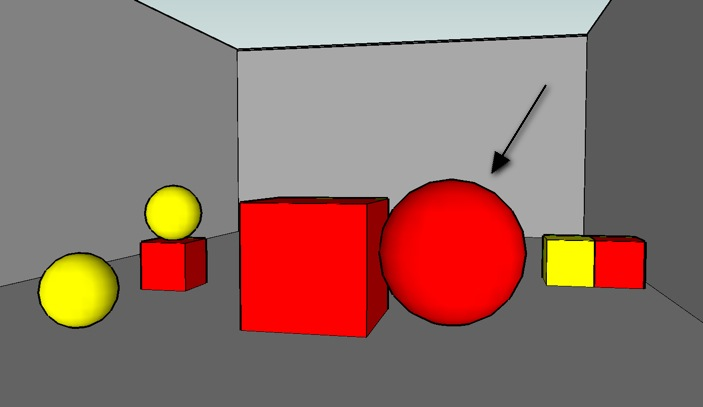
\includegraphics[scale=.4]{images/22sinletras.jpg}
\caption{Ejemplo de contexto}
\label{GRE3D7-stimulus1}

\end{figure}

%\setlength{\unitlength}{1cm}
%
%\newsavebox{\mybox} 
%\savebox{\mybox}{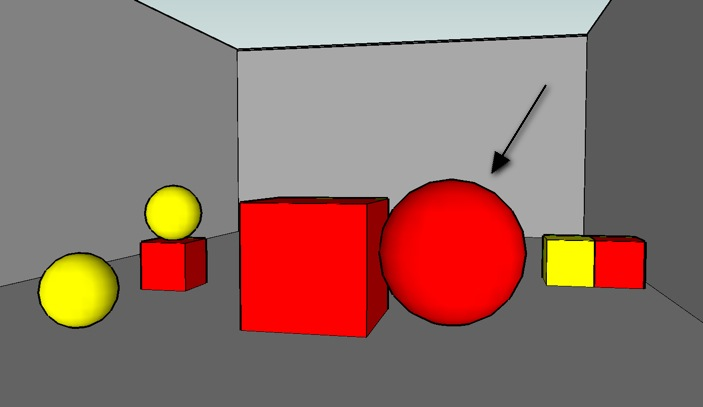
\includegraphics[scale=0.40]{images/22sinletras.jpg}\caption{Ejemplo de contexto}\label{GRE3D7-stimulus1}} 
 %\begin{figure}
   %\begin{picture}(8,6)
  %\put(0,0){\usebox{\mybox}} 
  %%\put(2,2.5){\oval(6,5)}
   %\end{picture}   
 %\end{figure}    

Una \emph{expresi\'on referencial} es una sintagna nominal que identifica univocamente al objeto target en un contexto considerado y para un interlocutor particular.

Si quisieramos referirnos al objeto se\~nalado por la flecha en la Figura~\ref{GRE3D7-stimulus1} podr\'iamos hacerlo con la expresi\'on referencial ``la
esfera roja que est\'a al lado del cubo rojo'', o ``la bola grande'' o ``el objeto que esta al lado del cubo grande''. 

\begin{figure}[ht]
\centering
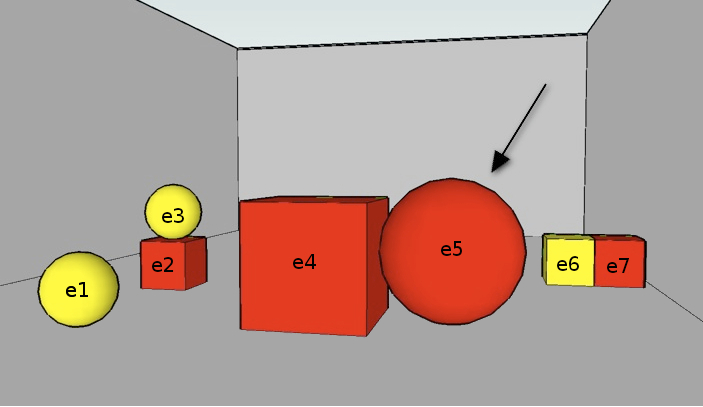
\includegraphics[width=0.6\textwidth]{images/22.jpg}
\caption{Ejemplo de contexto con objetos etiquetados}
\label{GRE3D7-stimulus2}
\end{figure}

%\setlength{\unitlength}{1cm}
%
%%\newsavebox{\mybox} 
%\savebox{\mybox}{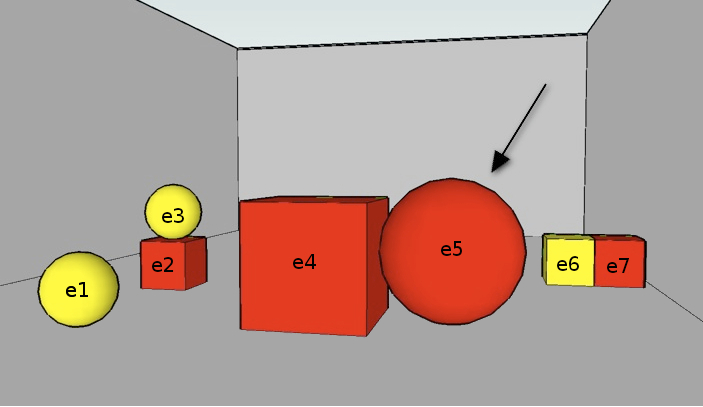
\includegraphics[scale=0.40]{images/22.jpg}\caption{Ejemplo de contexto con objetos etiquetados}\label{GRE3D7-stimulus2}} 
 %\begin{figure}
   %\begin{picture}(8,6)
  %\put(0,0){\usebox{\mybox}} 
  %%\put(2,2.5){\oval(6,5)}
   %\end{picture}   
 %\end{figure}    


Ahora imaginemos una computadora que se enfrenta a la misma
tarea, ella necesitar\'a tener a los objetos identificados y las propiedades de cada uno de ellos, una forma de identificar a los objetos se muestra en la Figura~\ref{GRE3D7-stimulus2}. Suponiendo que tiene acceso a una base de datos que contiene todas
las propiedades relevantes de los objetos de la escena, como se muestra en la Tabla \ref{tabla-propiedades}, la tarea de encontrar una ER para el objeto $e_5$ es lo mismo que encontrar alguna combinaci\'on de propiedades que se aplica \'unicamente a $e_5$, y no a los otros objetos.\\


\begin{table}[h!]
\begin{center}
\begin{tabular}{|l|c|c|c|c|c|c|}
\hline
%Figure & Model \puse &  Learning \puse & Random \puse &  Uniform \puse \\
Objeto& 	Forma		&	Color	&	Tama\~no & Al lado de & Arriba de	& Abajo de	\\
\hline
$e_1$ & esfera & amarillo & chico & - & - & -\\
$e_2$ & cubo & rojo & chico & - & - & $e_3$\\
$e_3$ & esfera & amarillo & chico & - & $e_2$ & -\\
$e_4$ & cubo & rojo & grande & $e_5$ & - & -\\
$e_5$ & esfera & rojo & grande & $e_4$ & - & -\\
$e_6$ & cubo & amarillo & chico & $e_7$ & - & -\\
$e_7$ & cubo & rojo & chico & $e_6$ & - & -\\

\hline
\end{tabular}
%\vspace*{.1cm}
\caption{Propiedades de los objeto de la Figura \ref{GRE3D7-stimulus2}.}
\vspace*{-.5cm}
\label{tabla-propiedades}
\end{center}
\end{table}
%\vspace*{-.5cm}


Esta tarea de encontrar las propiedades que aplican a un objeto y no a los otros, se llama selecci\'on de contenido de una expresi\'on referencial.  

Imaginemos una computadora con la informaci\'on de la Tabla \ref{tabla-propiedades} queriendo distinguir a $e_5$, puede que haya m\'as de una forma en la que $e_5$ puede ser distinguido del resto (``la esfera roja grande'', ``la esfera que esta al lado del cubo grande'', ``la esfera roja''), la computadora tiene que decidir cu\'al de esas expresiones referenciales es \'optima en el contexto dado. Por otra parte, el concepto de \'optimo puede significar diferentes cosas.

Se podr\'{i}a pensar, por ejemplo, que las referencias son \'optimas cuando son m\'{i}nimas en longitud, es decir, 
que contiene s\'olo la informaci\'on suficiente para identificar el objeto target. Pero, como veremos, la b\'usqueda de referencias m\'{i}nimas
es computacionalmente cara, y no es necesariamente lo que los hablantes hacen, ni lo que es m\'as \'util para los oyentes.

De todas las subtareas de GLN, la Generaci\'on de Expresiones Referenciales (GER) es
una de las que ha recibido m\'as atenci\'on. En la pr\'actica, la mayor\'ia de los
sistemas NLG, con independencia de su finalidad, contiene un m\'odulo GER de alg\'un tipo~\cite{Mellish2004}. Esto no es sorprendente
en vista del papel central que las expresiones referenciales en la comunicaci\'on. Un sistema que proporciona
consejos sobre los viajes a\'ereos \cite{white2010generating} ha de hacer referencia a los vuelos (``el
vuelo m\'as barato'', ``un vuelo directo''), un sistema de navegaci\'on para autom\'oviles~\cite{Drager:2012:GLN:2380816.2380908}
necesita para generar descripciones espaciales para las \'areas (``tomar el puente junto a la iglesia a la derecha''),
y un sistema de di\'alogo de un robot que ensambla piezas de juguetes, junto con un usuario humano~\cite{foster-etal-ijcai2009} ha de hacer referencia a los componentes (``inserte el perno verde hasta el final en el cubo rojo'').

El {\it dominio} define los tipos de entidades que est\'an siendo contemplados, en algunos
casos incluso un determinado conjunto de entidades con todas sus propiedades.

El {\it contexto} contiene un subconjunto de las entidades del dominio, por ejemplo, los puntos de referencia visibles en un cierto punto de la ruta para la que estamos dando direcciones, un subconjunto de las fotograf\'ias utilizadas en una configuraci\'on experimental, o los ingredientes de cocina que ya se han mencionado en una receta. En un entorno visual, el contexto, incluyendo las
propiedades de sus objetos y su configuraci\'on espacial, se puede llamar escena. 

Cada objeto o entidad tiene un tipo, ciertas propiedades o caracter\'isticas, valores de esas propiedades, y relaciones con otros objetos.

Una {\it propiedad} es una caracter\'istica de una entidad particular por ejemplo, la raza de un perro, el tener o no tener bigotes para un hombre, o el color para un objeto, cada entidad puede tener muchas propiedades, e incluso puede tener relaciones, as\'i como las relaciones familiares, las relaciones con respecto a la posici\'on f\'isica, por ejemplo: el hecho de estar situado al lado de otro objeto.

El \emph{target} (u objetivo), es el objeto al cual queremos referirnos. En la escena de nuestro ejemplo en la Figura \ref{GRE3D7-stimulus1} es el se\~nalado por la flecha.

Los \emph{distractores} son objetos que se encuentran en el contexto considerado, y por los cuales es necesario hacer una expresi\'on referencial para identificar a nuestro target. 

Un {\it algoritmo} para la generaci\'on autom\'atica de expresiones referenciales (GER), es un procedimiento que toma alg\'un tipo de base de datos que representa un contexto y un target, y d\'a como resultado una expresi\'on referencial.

Un algoritmo para la GER es \emph{no-determin\'istico} si puede dar diferentes ER para el mismo contexto y target en sucesivas ejecuciones.
En esta tesis estudiamos la generaci\'on autom\'atica de expresiones referenciales, 
primero mostramos c\'omo podemos a\~nadir no determinismo a los algoritmos estudiados. Los algoritmos de refinamiento estudiados, tienen un orden fijo en el cual consideran las propiedades y relaciones, y la naturalidad de las expresiones referenciales que generan depende de este orden particular considerado, nosotros proponemos reemplazar ese orden fijo sobre las propiedades y/o relaciones de la escena de entrada por una~\emph{probabilidad de uso} para cada propiedad y/o relaci\'on, y modificar los algoritmos para que tengan en cuenta esas propiedades. De esta manera, cada llamada al algoritmo puede producir diferentes ERs para la misma escena y target de entrada. 

Nuestra aproximaci\'on es emp\'irica, en el sentido de que para evaluar nuestros resultados, usaremos corpus (colecciones de datos) de expresiones referenciales hechas por humanos.

Es decir nuestra meta, no s\'olo ser\'a crear algoritmos para la generaci\'on autom\'atica de expresiones referenciales, sino crearlos de tal manera que podamos imitar en gran medida lo que dir\'ian las personas.

Mostraremos que dado un corpus (como el corpus GRE3D7 o el TUNA de los cuales hablaremos en Cap\'itulo~\ref{sec:seleccion}) podemos estimar estas probabilidades de uso de manera que las ER se generen con una distribuci\'on de probabilidad que coincide en gran medida con las que se encuentra en el corpus.




\section{Descripci\'on del problema}
\label{sec:problema}

En ling\"u\'{i}stica, una expresi\'on referencial ER (que viene de la expresi\'on en ingl\'es referring expression (RE)) es una expresi\'on que identifica un\'ivocamente a un objeto para un interlocutor particular, desde un conjunto de posibles distractores. Por ejemplo si nosotros queremos identificar a un cierto animal \texttt{d} de un conjunto de mascotas, la expresi\'on ``el perro'' ser\'a una ER si \texttt{d} es el \'unico perro en el conjunto, y si nosotros estamos seguros que nuestro interlocutor identificar\'a a \texttt{d} como un perro. Para una persona esto ser\'ia una tarea f\'acil de realizar, pensemos ahora como lo har\'ia una computadora, supongamos que queremos conseguir un algoritmo que genere autom\'aticamente esas expresiones referenciales que la gente genera.\\



 Para que una computadora pueda generar las ER generadas por las personas, primero deber\'ia seleccionar las propiedades y/o relaciones que se incluir\'an en la ER, deber\'a tener una base de datos conteniendo las propiedades y relaciones relevantes de la escena, podemos imaginar que una computadora podr\'a generar muchas m\'as expresiones referenciales que una persona, este es un desaf\'io que direccionaremos en esta tesis, nuestra meta ser\'a imitar al humano en la generaci\'on de expresiones referenciales. 

Esta selecci\'on de la ER m\'as apropiada tambi\'en debe tener en cuenta al interlocutor, es natural que los humanos demos distintas ER a distintos interlocutores. En el \'area muchas veces se habla de optimalidad de la ER, pero con diferentes significados, para algunos una ER \'optima es aquella que dice lo m\'inimo necesario para identificar al objeto target, para otros es la menos esfuerzo requiere del interlocutor para identificarlo.
La selecci\'on de qu\'e propiedades y/o relaciones con otros objetos incluir en una expresi\'on referencial depender\'a del prop\'osito que tengamos para dicha expresi\'on referencial. Una expresi\'on referencial ser\'a muy distinta si nuestro objetivo es dar la m\'inima informaci\'on que identifique al objeto que si nuestro objetivo es ayudar al interlocutor a que identifique el objeto.

En la vida real hay muchas cosas que nos ayudan a darnos cuenta si nuestro interlocutor identific\'o el objeto target, como ser la expresi\'on de duda nos dar\'ia una pauta de que no esta entendiendo lo que le queremos decir, pero cuando queremos hacer esa generaci\'on autom\'atica normalmente no poseemos esa clase de informaci\'on.

En esta tesis nos vamos a enfocar en la selecci\'on de contenidos de las expresiones referenciales, y el objetivo ser\'ia simular el comportamiento humano, para ello vamos a usar corpus de expresiones referenciales para aprender como realizan esta tarea las personas.
 
Las propiedades y relaciones de los objetos de la escena forman una base de conocimento (KB), estos datos se pueden organizar en jerarqu\'ias, por ejemplo: conjunto de animales, conjunto de mamiferos, conjunto de insectos. Algunos conjuntos pueden estar contenidos en otros, es decir algunos objetos o entidades pueden compartir caracter\'isticas.\\

Hay diferentes tipos de propiedades, por ejemplo taxon\'omicas (las que tiene el objeto, por ejemplo tipo, color), relacionales (las que necesitan dar una ER de otro objeto, por ejemplo ``estar al lado de...''), vagas (son las m\'as dificiles de identificar, ejemplo: chico, grande, no son propiedades absolutas).

Si el objeto target tiene la propiedad de medir 1.80 de alto, y est\'a en un grupo donde los dem\'as son m\'as peque\~nos, es m\'as natural decir el m\'as alto, que el que mide 1.80.\\

Si tenemos 100 caracter\'isticas de una persona, y con esas caracter\'isticas se pudiera identificar un\'ivocamente a una persona, un sistema que diera que las 100 caracter\'isticas no ser\'ia un sistema que suene muy natural, ya que una persona no dar\'ia 100 propiedades para identicar a una persona particular. As\'i podr\'iamos decir que las expresiones referenciales variaran seg\'un la cantidad de informaci\'on que dan, si dan la m\'inima informaci\'on para identificarlas un\'ivocamente ser\'an minimales, si dan m\'as informaci\'on estar\'an sobreespecificadas, pero en el caso de dar m\'as de la m\'inima informaci\'on... cu\'anta m\'as dar?, intentaremos imitar lo que hacen las personas cuando dan expresiones referenciales para responder este tipo de preguntas.\\

%El sistema deber\'ia tener una lista del orden de preferencia de los atributos a usar.\\ 

Ciertos tipos de atributos pueden ser m\'as f\'aciles de identificar que otros, por ejemplo cierto color verde podr\'{i}a ser m\'as complicado de identificar que el tama\~no. Notar que cuando decimos el tama\~no podemos decir ``grande'' y tenemos como marco de referencia a los objetos de la escena, en ese contexto un objeto es ``grande''.\\

%NO NO Las primeras investigaciones en GER no voy a poner esto porque no quiero pasar por alto shrdlu de vinogran 1969
\cite{C92-1038}; \cite{Dale95computationalinterpretations} hicieron una serie de supuestos simplificadores, por ejemplo no usaban relaciones, el target era un s\'olo objeto, y como resultado los primeros
algoritmos GER s\'olo pod\'ian generar una variedad limitada de expresiones referenciales. Cuando
los investigadores comenzaron a levantar algunos de estos supuestos, esto di\'o lugar a algoritmos de GER
con un repertorio m\'as amplio, siendo capaces de generar, por ejemplo, plurales y expresiones relacionales. \\

Este movimiento ha creado una serie de nuevos desaf\'ios, sin embargo. Por ejemplo, el
n\'umero de formas en las que uno puede referirse a un conjunto de objetos de destino aumenta, por lo que la elecci\'on de una
buena expresi\'on referencial es m\'as dif\'icil.\\

Del mismo modo, incluso propuestas recientes tienden a asumir que no es problem\'atico para determinar qu\'e informaci\'on
es compartida entre el hablante y el oyente.
 (a) C\'omo se representa la informaci\'on del dominio?
(b) C\'omo se representa el contenido sem\'antico de una expresi\'on referencial? y (c) C\'omo se pueden encontrar descripciones distintivas?.\\

 En los contextos de los corpus analizados en esta tesis, nos encontramos con cuatro tipos diferentes de atributos:
tipos de objetos, atributos absolutos, atributos relativos y atributos espaciales incluidas las relaciones y atributos de localizaci\'on.\\

El tipo de un objeto constituye un caso especial, ya que es muy rara vez omite
en la expresi\'on referencial. En consecuencia, la mayor\'ia de los algoritmos tratan de
considerarlo por separado para asegurarse de que se a\~nade a cada expresi\'on referencial. \\

Una explicaci\'on parcial para esta condici\'on especial es que las expresiones referenciales consiguen realizarse como sintagmas nominales,
cada sintagma nominal requiere un sustantivo, y por lo general es el tipo del referente dado que es el sustantivo principal.\\

%\section{Contribuciones de esta tesis}
%\label{sec:contribiciones}
%\textcolor{blue}{Esta parte se va?}
%\begin{itemize}
%\item Se estudi\'o el avance en el \'area de la generaci\'on autom\'atica de expresiones referenciales, los algoritmos existentes y los problemas que ellos ten\'ian, las aproximaciones emp\'iricas realizadas en el \'area en el Cap\'itulo~\ref{sec:seleccion}.
%\item Se estudiaron las m\'etricas de evaluaci\'on tanto autom\'aticas como manuales en el Cap\'itulo~\ref{sec:seleccion}, las cuales ser\'an luego aplicadas en el Cap\'itulo~\ref{sec:evaluacion}.
%%\item Se abordaron los siguientes problemas: no-determinismo, sobreespecificaci\'on.
%\item Se estudiaron estudiaron distintas l\'ogicas y sus lenguajes asociados, se compararon esos lenguajes con el lenguaje utilizado para dar ER, a fin de elegir una l\'ogica apropiada en el Cap\'itulo~\ref{sec:intro_logica}.
%\item Se seleccion\'o un algoritmo existente al cual se le agregaron probabilidades de uso para simular el no-determinismo encontrado en corpus. Este fue seleccionado por permitirmos agregar los aspectos tenidos en cuenta en esta tesis: dar un algoritmo que aborde el no-determinismo, la sobreespecificaci\'on que sea relacional, que genere plurales en el Cap\'itulo~\ref{sec:learning}.
%%\item Se modific\'o el algoritmo para que sea no-determinista.
%\item Se agreg\'o sobreespecificaci\'on al algoritmo permitiendo agregar propiedades o relaciones cuando estas tienen una alta probabilidad de uso en corpus. Y al mismo tiempo se agura la terminaci\'on en el Cap\'itulo~\ref{sec:algoritmo}.
%\item Se propone un m\'etodo para calcular las probabilidades de uso (\puse)\ de las relaciones del modelo el cual genera una distribuci\'on de expresiones referenciales cercana a la encontrada en el corpus.
%\item Se prob\'o el algoritmo en 2 corpus existentes (el GRE3D7 y el Tuna corpus) en el Cap\'itulo~\ref{sec:evaluacion}.
%\item Se realiz\'o una evaluaci\'on en la que se compararon las salidas del algoritmo con ambos corpus. Se usaron m\'etricas autom\'aticas y manuales Cap\'itulo~\ref{sec:evaluacion}.
%\item Se creo un corpus de descripciones de mapas (el ZOOM corpus).
%\item Se hizo un caso de estudio de 3 mapas del ZOOM corpus explicado en Cap\'itulo~\ref{sec:corpus}, en el cual se toma 1 mapa con target singular, el mismo mapa con zoom 2x y target singular y el mismo mapa con target plural.
%\end{itemize}

\section{Mapa de la tesis}
\label{sec:mapadetesis}
\paragraph{Cap\'itulo~\ref{sec:intro}: ``Introducci\'on a la expresi\'on referencial''} Situamos a la generaci\'on autom\'atica de expresiones 
referenciales dentro de la inteligencia artificial y de la generaci\'on de lenguaje natural. Luego dimos las partes de un sistema de 
generaci\'on de lenguaje natural, el cual incluye la generaci\'on de expresiones referenciales y por lo tanto, \'este ultimo tiene las mismas 
partes principales. Entre esas partes est\'a la determinaci\'on de contenido, que es la selecci\'on de las propiedades que vamos a elegir 
para identificar un\'ivocamente al objeto de los dem\'as objetos del contexto, sobre este tema, trabajaremos profundamente en el resto de la 
tesis. Dimos intuiciones de qu\'e es una expresi\'on referencial en el contexto de una imagen que presentamos. Despu\'es explicamos la 
importancia de la generaci\'on de expresiones referenciales dentro de la generaci\'on de lenguaje natural, en 
dominios diferentes que van desde generaci\'on de pron\'osticos del tiempo, resumir informaci\'on m\'edica, dar consejos de viajes a\'ereos, 
sistemas de apoyo para la contrucci\'on de juguetes... en fin... {\it D\'igame un sistema, y puedo decirle donde usa expresiones 
referenciales!}. Explicamos conceptos b\'asicos que usaremos a lo largo de la tesis, como ser el de {\it dominio}, {\it contexto}, 
{\it propiedad}, {\it target}, {\it distractor} y {\it algoritmo}. Dimos una introducci\'on a la variedad de expresiones referenciales que 
se puede tener para el mismo objeto target en el mismo contexto.

\paragraph{Cap\'itulo~\ref{sec:seleccion}: ``Generaci\'on de expresiones referenciales''} Formalizamos los diferentes tipos de expresiones referenciales: proposicionales, relacionales, minimales, sobreespecificadas, subespecificadas, los diferentes tipos de algoritmos para la tarea de generaci\'on autom\'atica de expresiones referenciales: determin\'isticos, no-determin\'isticos, que generan sobreespecificaci\'on, 
plurales, s\'olo singulares, relacionales o proposicionales, los algoritmos tambi\'en se pueden distinguir por la forma en la que toman el 
input: mostramos un ejemplo de input de 2 algoritmos conocidos de la literatura, la forma en la que deciden cu\'al propiedad o relaci\'on 
agregar es decir la teor\'ia subyascente del algoritmo. Se estudi\'o el avance en el \'area de la generaci\'on autom\'atica de expresiones referenciales, los algoritmos existentes y los problemas que ellos ten\'ian, las aproximaciones emp\'iricas realizadas en el \'area.
%Luego se explica la historia de los algoritmos del \'area de generaci\'on autom\'atica
% de expresiones referenciales. 
Despu\'es vemos que una forma de acercarnos m\'as a la generaci\'on autom\'atica de expresiones referenciales  imitando el comportamiento humano, es viendo c\'omo los humanos hacen expresiones referenciales, llamamos {\it aproximaciones emp\'iricas} a aquellos algoritmos que hacen uso de corpus de expresiones referenciales dichas por humanos. Damos una breve descripci\'on de los corpus que actualmente hay disponibles en el \'area y al ver la simplicidad de estos corpus, por un lado podemos ver la complejidad de la tarea, ya que si para corpus tan simples, es tan dif\'icil conseguir algoritmos que hagan lo que hacen los humanos, podr\'iamos imaginarnos que es realmente una tarea mucho m\'as dif\'icil en contextos que la gente usa en la vida diaria, y por otro lado, motivamos la obtenci\'on de un nuevo  corpus, el cual describiremos en el Cap\'itulo \ref{sec:corpus}, el cual usa im\'agenes de mapas de ciudades como contexto. Para finalizar damos una introducci\'on a las m\'etricas de evaluaci\'on. 

%Habiendo ya decidido cuales son los tipos de expresiones referenciales que queremos generar en el Cap\'itulo \ref{sec:seleccion} y ya teniendo 
%claro el lenguaje \EL que hemos seleccionado en el Cap\'itulo \ref{sec:intro_logica}, en el 

\paragraph{Cap\'itulo~\ref{sec:intro_logica}: ``Introducci\'on a la L-simulaci\'on''} En este cap\'itulo nuestra meta es seleccionar una l\'ogica cuyo lenguaje sea apropiado a nuestro problema de generaci\'on de expresiones referenciales que imite el comportamiento humano. Cada l\'ogica tiene una sem\'antica particular, la cual genera un cierto lenguaje. Partimos desde la l\'ogica de primer orden (\FOL), la m\'as amplia, explicamos el lenguaje asociado, para darnos una idea de cuales son las f\'ormulas que el lenguaje puede generar, vemos una serie de ejemplos de f\'ormulas que se pueden generar con ese lenguaje y si podemos compararlas con las expresiones referenciales que dar\'ia un humano. Luego vemos l\'ogicas con menos poder expresivo como \EPFOL (\FOL sin negaci\'on), \ALC, \EL, \ELAN \textcolor{blue}{ACA FALTA!!} y seleccionamos como nuestro lenguaje el \EL y justificamos nuestra selecci\'on. Daremos definiciones b\'asicas de modelo, interpretaci\'on, f\'ormula, hablaremos de la noci\'on de similaridad de 2 elementos u y v del modelo la cual dice que son L-similares ($u \simil{\+L} v$ en el lenguaje $L$), cuando para toda f\'ormula $\gamma \in L$, tenemos que $\{u,v\} \subseteq \interp{\gamma}$, se dice que no podemos identificarlos por separado, ya que no hay una f\'ormula que satisfaga uno y no el otro, es decir es lo que usaremos para saber cuales son las propiedades y relaciones de una ER para un target particular. Veremos un teorema que acota el ``para todo'' antes mencionado, el cual nos permitir\'a chequear un conjunto finito de f\'ormulas para saber que hay una ER para el target, es decir que no existe otro elemento en el modelo el cual sea una $\simil{\+L}$ al target. 
%Si pudieramos identificar a un elemento de los dem\'as con una f\'ormula diremos que es la expresi\'on referencial para ese elemento en ese 
%lenguaje. \cite{arec:usin11} dicen que dados dos modelos$\tup{\Delta_1, \interp{\cdot}_1}$ and $\tup{\Delta_2,
%\interp{\cdot}_2}$, consideremos las siguiente
%propiedades de una relaci\'on binaria ${\sim} \subseteq \Delta_1 \times \Delta_2$ Diremos que una relaci\'on binaria no-vac\'ia $\sim$ es una 
%\emph{$\+L$-simulacion} cuando satisface ciertas propiedades que dependen del lenguaje considerado, es decir de la l\'ogica considerada, 
%diremos que un objeto
%\emph{$v$ $\+L$-simula $u$} (notaci\'on $u \simul{\+L} v$) si hay una relaci\'on $\sim$ que satisface el correspondientes propiedades tal que
%$u \sim v$. Un teorema dice que Si $\+M_1 = \tup{\Delta_1, \interp{\cdot}_1}$ and $\+M_2 =
%\tup{\Delta_2, \interp{\cdot}_2}$ son modelos finitos, $u \in \Delta_1$ and $v \in \Delta_2$, entonces $u \simil{\+L} v$ si y s\'olo si 
%$u \simul{\+L} v$ (para $\+L \in \cset{\FOL,\EPFOL,\ALC,\EL,\ELAN}$). Se presentan los algoritmos...
%

\paragraph{Cap\'itulo~\ref{sec:algoritmo} ``Nuestra propuesta''} Habiendo ya decidido cu\'ales son los tipos de expresiones referenciales que queremos generar en el Cap\'itulo \ref{sec:seleccion} y ya teniendo
claro el lenguaje \EL que hemos seleccionado en el Cap\'itulo \ref{sec:intro_logica}, en este cap\'itulo 
explicamos nuestra propuesta de agregar probabilidades de uso a las palabras de la signatura del modelo, adaptando un algoritmo existente 
\cite{arec2:2008:Areces} el cual introducimos en \ref{sec:seleccion}, modificamos el algoritmo permitiendo sobreespecificaci\'on, 
pero asegurando terminaci\'on y agregamos un componente aleatorio para conseguir no-determinismo. Mostramos en detalle el input que toma el
 nuevo algoritmo, dejando como caja negra de d\'onde la sacamos las probabilidades de uso, tema que abordaremos en el siguiente cap\'itulo. 
Mostramos la salida del algoritmo, explicamos c\'omo conseguimos no-determinismo en las distintas ejecusiones del algoritmo, como aseguramos 
terminaci\'on. Adem\'as mostramos completitud, es decir que siempre conseguimos la expresi\'on referencial si existe. Explicamos como agregamos sobreespecificaci\'on a las expresiones referenciales. Luego damos un ejemplo de ejecuci\'on. 


\paragraph{Cap\'itulo~\ref{sec:learning}: ``Probabilidades de uso''} Explicamos como obtener las probabilidades de uso usadas por el algoritmo del Cap\'itulo \ref{sec:algoritmo} a partir de corpus cuando hay disponible o una aproximaci\'on usando aprendizaje autom\'atico cuando no hay corpus disponible para la escena y target considerados. Para aprendizaje autom\'atico usamos caracter\'isticas simples y vemos que son buenas, es decir conseguimos probabilidades de uso que hacen que las ejecusiones del algoritmo consigan ERs como las del corpus, pero tambi\'en descubrimos cosas que no podemos aprender, como por ejemplo que \textcolor{blue}{ACA FALTA!! }

\paragraph{Cap\'itulo~\ref{sec:evaluacion}: ``Evaluaci\'on de nuestra propuesta''} En esta tesis se estudiaron las m\'etricas de evaluaci\'on tanto autom\'aticas como manuales. Evaluamos nuestro algoritmo, teniendo en cuenta ambos tipos de m\'etricas. La evaluaci\'on esta dividida en 2 partes. Una parte en la cual comparamos la salida del algoritmo para modelos de los 2 corpus estudiados en el Cap\'itulo \ref{sec:seleccion} con las expresiones referenciales dadas por los humanos, con ejecusiones del algoritmo tomando probabilidades de uso sacadas del mismo corpus, obtenidas con aprendizaje autom\'atico a partir del corpus, aleatorias y con la distribuci\'on uniforme de las ER dadas por las personas, mostramos la entrop\'ia cruzada entre ellos. Vemos como las probabilidades aprendidas del corpus y con aprendizaje autom\'atico se acercan mucho m\'as al corpus, que las random o unifomes. Y la otra parte una evaluaci\'on manual en la cual pusimos a 2 jueces a decidir cual ER era mejor, o pod\'ian considerarlas igual de buenas, si la del corpus, o la generada por el algoritmo, es interesante notar como muchas veces las ER generadas por el algoritmo eran mejores que las humanas!, el algoritmo tiene la ventaja que siempre da una ER si existe, en cambio los humanos muchas veces dan expresiones ambiguas que no son referenciales. Notamos que al usar las probabilidades aprendidas desde el corpus el algoritmo da ER que son las del top ranking de las personas.

\paragraph{Cap\'itulo~\ref{sec:corpus}: ``Recolecci\'on y an\'alisis del corpus ZOOM''} Introducimos un nuevo corpus, el ZOOM corpus, el cual fue recolectado en un trabajo conjunto con la Universidad de S\H ao Paulo Brasil, para tener un corpus m\'as natural de expresiones refenciales ya que el corpus nombrado tiene expresiones referenciales de mapas. Los mapas son fragmentos de las ciudades de Madrid y Lisboa. Este corpus fue recolectado en 2 idiomas, espa\~nol y portugues. Se explica el m\'etodo de recolecci\'on del corpus, se dan estad\'isticas de las personas que completaron el experimento, se explica la manera en que se anot\'o el corpus y se da una evaluaci\'on del corpus conseguido. caso de estudio de 3 mapas del ZOOM corpus explicado en Cap\'itulo \ref{sec:corpus}, en el cual estudiamos un mapa con 1 target sin zoom, el mismo mapa pero zoom 2X, y el mismo mapa pero como 2 targets. Mostramos como funciona el algoritmo para un caso tan real y natural como son los mapas del ZOOM corpus. 


\paragraph{Cap\'itulo~\ref{sec:conclusiones}: ``Conclusiones''} Se resumen lo estudiado y realizado en esta tesis, se explican las cosas aprendidas, y dan l\'ineas de trabajo futuro. \textcolor{blue}{ACA FALTA!! }

